\documentclass[]{spie}  %>>> use for US letter paper
%\documentclass[a4paper]{spie}  %>>> use this instead for A4 paper
%\documentclass[nocompress]{spie}  %>>> to avoid compression of citations

\renewcommand{\baselinestretch}{1.0} % Change to 1.65 for double spacing
 
\usepackage{amsmath,amsfonts,amssymb}
\usepackage{graphicx}
\usepackage[colorlinks=true, allcolors=blue]{hyperref}


\usepackage{color}
\usepackage[latin9]{inputenc}
\usepackage{mathrsfs,amsmath}
\usepackage{graphicx}%
\usepackage{float}
\usepackage{amsfonts}%
\usepackage[titletoc]{appendix}
\usepackage{amssymb}
\usepackage{braket}
\usepackage{bm}

\newcommand{\mb}[1]{\bm{#1}}
\usepackage[T1]{fontenc}

\def\Nabla{\bm{\nabla}}
\def\bm{\mathbf}
\def\curl{\Nabla\times}
\def\div{\Nabla\cdot}
\def\lap{\Delta}
\def\vlap{\Delta}
\def\x{\hat{e}_{x}}
\def\y{\hat{e}_{y}}
\def\z{\hat{e}_{z}}
\def\p{\partial}
\def\h{\hat}
\DeclareMathOperator{\Tr}{Tr}


\title{Temporal Hole Burning in QCLs with strong injector anticrossing}


\author[a]{Petar Tzenov}
\author[b]{David Burghoff}
\author[b]{Qing Hu}
\author[a]{Christian Jirauschek}
\affil[a]{Institute for Nanoelectronics, Technical University of Munich, D-80333 Munich, Germany}
\affil[b]{Department of Electrical Engineering and Computer Science, Research Laboratory of Electronics, Massachusetts Institute of Technology, Cambridge, Massachusetts 02139, USA}
\date{June 6, 2016}%

\authorinfo{Further author information:\\a: E-mail: petar.tzenov@tum.de}

% Option to view page numbers
\pagestyle{empty} % change to \pagestyle{plain} for page numbers   
\setcounter{page}{301} % Set start page numbering at e.g. 301
 
\begin{document} 
\maketitle


\begin{abstract}
In this work we investigate the temporal dynamics of terahertz (THz) quantum cascade lasers (QCL) with a strong injector anticrossing via numerical solution of the Maxwell-Bloch laser equations.
The presence of a strong anticrossing between the injector and upper laser levels in typical longitudinal optical phonon THz QCL designs, has been shown to lead to a pronounced splitting of the emission spectra into high and low frequency lobe components around the central frequency of several THz. Until recently however, the time domain implications of such spectral hole burning effect had not been considered. Here we present a theoretical explaination of this "temporal hole burning" phenomena, simulation results which illustrate it and also experimental evidence which support our claims. 
\end{abstract}

% Include a list of keywords after the abstract 
\keywords{THz QCLs, temporal hole burning, density matrix model}

\section{Introduction}
Quantum cascade lasers (QCLs) are promising candidates for compact sources of coherent radiation in the far and mid- infrared regions of the electromagnetic spectrum. To name a few, practical applications of these type of devices range from spectroscopy and optical metrology in the area of fundamental sciences, non-invasive diagnostics (e.g. breath analysis) in medicine, to explosive detection for military applications. Furthermore, QCLs have shown to possess rich dynamics, such as spatial\cite{gordon2008multimode} and spectral\cite{burghoff2014terahertz} hole burning, multimode Risken-Nummedahl-Graham-Haken \cite{risken1968self,gordon2008multimode} instabilities,  as well as nonlinear processes such as self-phase modulation and four wave mixing \cite{friedli2013four,khurgin2014coherent}, which makes them extremely interesting from purely academic point of view.

In this proceedings, we will investigate a new type of phenomena, the so called "temporal hole burning" \cite{burghoff2015evaluating}, which is a form of pulse-switching behaviour in QCLs with strongly anticrossed gain. We will outline the system of equations which captures this effect and show a fully numerical solution thereof, where we also investigate parametric ranges where this intricate dynamics can be observed. Finally, we compare our simulations with experimental data followed by a discussion of possible applications for time-domain characterization of frequency combs.
\section{Experimental evidence}

Put David's measurements here. Evaluate the effect 


\section{Three-level system's density matrix equations}
Let us assume a simplified quantum cascade laser module consisting of only three relevant levels per period, the upper laser level $\ket{3}$, the lower laser level $\ket{2}$ and the depopulation level $\ket{1}$. This simple system can be taken as a basic example of resonant tunneling injection QCL, where the electrons are selectively injected into the upper laser level via a resonant tunneling process where the depopulation level of the previous period, also known as the injector level ( which we will denote by $\ket{1'}$ ), is at or near resonance with the upper laser level of the current module. Such a configuration provides a very effective current injection into the system and has been shown to significantly improve the device's performance CITE CITE CITE. 

To treat the resonant tunneling transition quantum mechanically, a theoretical approach beyond the standard two level Bloch equations is necessary. Here we outline the basic Hamiltonian, taken in the rotating wave approximation (RWA), which describes this microscopic system, coupled to the Maxwell's equations to model the effect of atomic polarization onto the total electric field. We set up the equations in the tight-binding approximation \cite{bastardwave}, where the energetic coupling between the states $\ket{1'}$ and $\ket{3}$ is characterized by the anticrossing energy $\hbar \Omega_{1'3}$ and the radiative coupling between the upper and the lower laser levels is written down in the electric dipole approximation with coupling energy equal to $q_0d_{32}E(x,t)$, where $q_0$ is the elementary charge, $d_{32}$ the transition dipole element and $E(x,t)$ the electric field. A schematic illustration of the described configuration, with the wave functions calculated in the tight-binding basis, is depicted in Fig. \ref{fig:3lvlsystem}.
\begin{figure}[h!]
	\begin{center}
		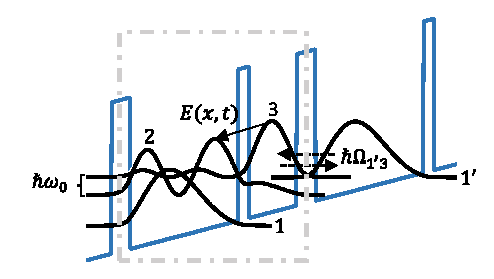
\includegraphics[scale=1]{IMGS/TOY3LVLSYSTEM.eps}
		\caption{ Insert Caption HERE} \label{fig:3lvlsystem}
	\end{center}	
\end{figure}
From the above discussion we have total of 4 discrete energy levels, $\ket{1'},\ket{3},\ket{2}$ and $\ket{1}$. In order to close the system we also employ periodic boundary conditions, by assuming that the depopulation level $\ket{1}$ is identical to the injector level $\ket{1'}$. This implies that we can effectively reduce the system to three relevant levels. In order to correctly capture the electron tunneling injection into the system, we set those levels to be the triplet $\ket{1'},\ket{3}$ and $\ket{2}$ \cite{callebaut2005importance,kumar2009coherence}. In operator form, the Hamiltonian of this toy system, in the rotating wave approximation reads 
\begin{align}
\label{eq:hamiltonian-operatorform}
\h{H}^{\text{RWA}} &= \hbar(\epsilon + \Delta) \h\sigma_{1',1'} +\hbar\Delta\h\sigma_{3,3} +(\hbar\Omega_{1'3}\h\sigma_{1',3} +\frac{q_0d_{32}}{2}f \h\sigma_{3,2}+h.c.),
\end{align}
where we have made the familiar ansatz decomposing the electric field $E(x,t) = \Re\{f(x,t) e^{i(k_cx-\omega_c t)}\}$ into the product of an envelope function $f(x,t)$ and a carrier wave with central angular frequency $\omega_c$ and wave number $k_c = n_0\omega_c/c$, given a background refractive index $n_0$ and the velocity of light in vacuum $c$. Also we have set  $\Delta = \omega_0 -\omega_c$, as the detuning of the electric field from $3\leftrightarrow 2$ resonance, $\hbar\omega_0 = E_3-E_2$ is the energy difference between levels $3$ and $2$, $\hbar\epsilon = E_{1'}-E_{3}$ is the tunneling level's detuning and we have also set the zero energy to be equal to the energy of the lower level $E_2 = 0$. Finally, $\h \sigma_{i,j}$ denotes the atomic projection operators and "$h.c$" the hermitian conjugate. 

%Taking the states $\Ket{1'},\Ket{3}$ and $\Ket{2}$ as a complete orthonormal basis, the Hamiltonian in Eq. (\ref{eq:hamiltonian-operatorform}) can be cast into matrix form as
%\begin{align}
% \label{eq:hamiltonian-matrixform}
% H^{\text{RWA}} &= \begin{pmatrix}
% \hbar(\epsilon + \Delta) & \hbar \Omega_{1'3} & 0 \\ 
% \hbar \Omega_{1'3} & \hbar\Delta & q_0d_{32}f/2 \\
% 0 & q_0d_{eg}f^*/2 & 0
% \end{pmatrix}.
% \end{align}
%Similarly, the density matrix (in the RWA) now reads
%\begin{align}
%\label{eq:DM-matrixform}
%\rho^{\text{RWA}} &= \begin{pmatrix}
%\rho_{1'1'} & \rho_{1'3} & \eta_{1'2} \\ 
%\rho_{31'} & \rho_{33} & \eta_{32} \\ 
%\eta_{21'} & \eta_{23} & \rho_{22} \\ 
%\end{pmatrix},
%\end{align}
%where we have taken that $\rho_{32} = \eta_{32}e^{i(k_cx-\omega_c t)}$ and $ \rho_{1'2} = \eta_{1'2}e^{i(k_cx-\omega_c t)}$.
The time evolution of the density operator $\h{\rho}^{\text{RWA}}$ (in the RWA) is governed by the von Neumann equation with phenomenologically included dissipation term $G(\h{\rho}^{\text{RWA}})$ and is given by
\begin{equation}
\label{eq:vonNeumann}
\frac{d \h{\rho}^{\text{RWA}}}{dt} = -\frac{i}{\hbar}[\h{H}^{\text{RWA}};\h{\rho}^{\text{RWA}}] + G(\h{\rho}^{\text{RWA}}).
\end{equation}
We will deter the discussion about the form of $G(\h\rho^{\text{RWA}})$ until Sec. \ref{sec:number} of this work. 
\section{Density matrix equations in the dressed states basis}
\begin{figure}[h!]
	\begin{center}
		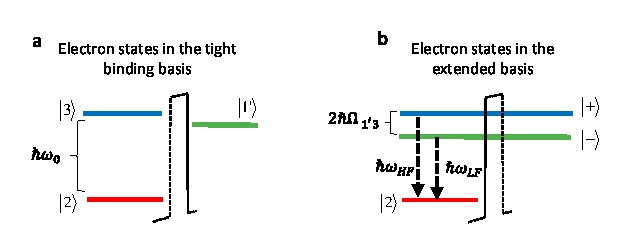
\includegraphics[scale=1]{IMGS/BASISPICTURE.eps}
		\caption{ Schematic illustration of the tight binding \textbf{a} and extended basis \textbf{b}, states.  } \label{fig:basis_schemata}
	\end{center}	
\end{figure}
 
 The introduction of the coupling energy $\hbar \Omega_{1'3}$ into the Hamiltonian of the system contributes to a splitting of the optical spectra into a high and a low frequency lobes. This is due to the fact that the extended system's Hamiltonian is non-diagonal in the tight binding basis. The new eigenstates, which in the absence of electromagnetic radiation, i.e. $f(x,t) \approx 0$, diagonalize the Hamiltonian in Eq. (\ref{eq:hamiltonian-operatorform}), are the so called dressed states and are obtained from the tunneling levels $\Ket{1'}$ and $\Ket{3}$ via the unitary transformation
 \begin{align}
 \label{eq:dressedstates}
 \Ket{+} &= \cos\theta \Ket{1'} - \sin\theta \Ket{3}, \nonumber \\
 \Ket{-} &= \sin\theta \Ket{1'} + \cos\theta \Ket{3}.
 \end{align}
 The corresponding energies are given by $E_\pm =\hbar(\omega_0 +\epsilon/2) \pm \hbar \left(\epsilon^2+4\Omega_{1'3}^2\right )^{1/2}$, and the expansion coefficients are computed from   
 $
 \tan \theta = -2\Omega_{1'3}/[\epsilon+(\epsilon^2+4\Omega_{1'3}^2)^{1/2}].
 $
 Within the full extended basis picture, where the wave functions are calculated for several neighbouring periods, these tight-binding states are simply split electron states spanning the intermodule barrier, see Fig. \ref{fig:basis_schemata}b. Both dressed states  couple radiatively to the lower laser level $\ket{2}$, since they both have a component in the $\ket{3}$ direction in the tight binding expansion. We can calculate the ratio of the dipole matrix elements for the $\Ket{+}\leftrightarrow\Ket{2}$ and $\Ket{-}\leftrightarrow\Ket{2}$ transitions, which will determine the relative strength between the high and low frequency lobes of the gain. If we assume that the $d_{1'2} \approx 0$, which is reasonable in the tight binding basis due to the negligible overlap between wave function in different modules, we obtain  $|\Bra{+}\hat{z}\Ket{2}|/|\Bra{-}\hat{z}\Ket{2} | \approx |\tan\theta| =  2|\Omega_{1'3}|/|\epsilon+\sqrt{\epsilon^2+4\Omega_{1'3}^2}|$. We now can see that at positive detunings $\epsilon >0$, $|\tan\theta|<1$ and thus the low frequency transition will have higher probability. On the other hand, for $\epsilon < 0 $ we get that $|\tan\theta| >1$ which will lead to lasing predominantly in the high frequency regime.
  
To see the origin of the temporal hole burning phenomena, we will apply the unitary transformation given by Eq. (\ref{eq:dressedstates}) into Eq. (\ref{eq:hamiltonian-operatorform}), i.e. we switch to the dressed state basis $\ket{+},\ket{-},\ket{2}$ to obtain the matrix
\begin{equation}
H = \begin{bmatrix}
\hbar \omega_+ & 0 & q_0d_{+2}E \\
0 & \hbar \omega_- & q_0d_{-2}E \\
q_0d_{+2}E & q_0d_{-2}E & 0 \\
\end{bmatrix}.
\end{equation}
Assuming the rotating wave approximation we get the following expressions for the Hamiltonian and the statistical operator
\begin{equation}
H^{\text{RWA}} = \begin{bmatrix}
\hbar (\omega_+-\omega_c) & 0 & q_0d_{+2}f/2 \\
0 & \hbar (\omega_--\omega_c) & q_0d_{-2}f/2 \\
q_0d_{+2}f^*/2 & q_0d_{-2}f^*/2 & 0 \\
\end{bmatrix},\quad \rho^{\text{RWA}} = \begin{pmatrix}
\rho_{++} & \rho_{+-} & \eta_{+2} \\ 
\rho_{-+} & \rho_{--} & \eta_{-2} \\ 
\eta_{2+} & \eta_{2-} & \rho_{22} \\ 
\end{pmatrix}.
\end{equation}
The symbols $d_{+2} = \Bra{+}\hat{z}\Ket{2} = -\sin\theta \Bra{3}\hat{z}\Ket{2}$ and $d_{-2} = \Bra{-}\hat{z}\Ket{2} = \cos\theta \Bra{3}\hat{z}\Ket{2}$, denote the corresponding dipole moments, and $\rho_{\pm 2} = \eta_{\pm 2} e^{i(k_cx-\omega_c t)}$. In this basis the von Neumann equation, Eq. (\ref{eq:vonNeumann}), reads (neglecting collision terms)
\begin{align}
\frac{d \rho_{++}}{dt} &= i\frac{q_0d_{+2}}{2\hbar}(f^*\eta_{+2}-f\eta_{+2}^*), \\
\frac{d \rho_{--}}{dt} &= i\frac{q_0d_{-2}}{2\hbar}(f^*\eta_{-2}-f\eta_{-2}^*), \\
\frac{d \rho_{22}}{dt} &= -i\frac{q_0d_{+2}}{2\hbar}(f^*\eta_{+2}-f\eta_{+2}^*)-i\frac{q_0d_{-2}}{2\hbar}(f^*\eta_{-2}-f\eta_{-2}^*), \\
\frac{d \rho_{+-}}{dt} &= -i(\omega_+-\omega_-)\rho_{+-}-i\frac{q_0d_{+2}}{2\hbar}f\eta_{2-}+i\frac{q_0d_{-2}}{2\hbar}f^*\eta_{+3},\\
\frac{d \eta_{+2}}{dt} &= -i(\omega_+-\omega_0)\eta_{+2}+i\frac{q_0d_{+2}}{2\hbar}f(\rho_{++}-\rho_{22})+i\frac{q_0d_{-2}}{2\hbar}f\rho_{+-},\\
\frac{d \eta_{-2}}{dt} &= -i(\omega_--\omega_0)\eta_{-2}+i\frac{q_0d_{-2}}{2\hbar}f(\rho_{--}-\rho_{22})+i\frac{q_0d_{+2}}{2\hbar}f\rho_{-+}.
\end{align}

Now If we assume that $f = f^*$, i.e. that the electric field envelope is real, $\epsilon \approx 0$, set that $d_{+2}\approx d_{-2} = d$ and substitute $\eta = \eta_{+2}+(\eta_{-2})^*$, the time evolution of $\eta$ is governed by
\begin{equation}
\label{eq:coherence_quasi2lvl}
\frac{d \eta}{dt} = -2i\Omega_{1'3} \eta + i\frac{q_0d}{2\hbar}fw, 
\end{equation}
where $w = \rho_{++}-\rho_{--}$ denotes the inversion between the dressed states, which evolves in time via 
\begin{align}
\label{eq:inversion_quasi2lvl}
\frac{d w }{dt}	&=  i\frac{q_0d}{2\hbar}f(\eta-\eta^*).
\end{align}
We thus see that under the above idealized assumptions, we have reduced the three level system into an effective two level such. In fact, this is a "quasi" two level system due to the presence of a factor of 2 in the denominator of Eq. (\ref{eq:inversion_quasi2lvl}), which distinguishes it from the standard Bloch equations \cite{boyd2003nonlinear}.

To see why Eqs. (\ref{eq:coherence_quasi2lvl}) and (\ref{eq:inversion_quasi2lvl}) could lead to a pulse switching behaviour we need to include the optical field propagation equations into the model. For classical fields, absence of free electric charges and weak inhomogenities, the electric field envelope (within the slowly varying amplitude approximation) obeys the propagation equation
\begin{align}
	\frac{n_0}{c} \p_t f - \p_x f = -i\frac{N \Gamma q_0d k_c}{\epsilon_0 n^2}(\eta_{+2}+\eta_{-2}),
\end{align}
where $\epsilon_0$ is the permittivity of free space and $N$ is the average carrier density per unit volume. Now decomposing the polarization envelopes, $\eta_{+2}$ and $\eta_{-2}$ into their real and imaginary parts, i.e. $\eta_{+2} = u_{+}+iv_{+}$ and $\eta_{-2} = u_{-}+iv_{-}$, and plugging into the propagation equation we obtain that
\begin{align}
\label{eq:field_propagation}
\frac{n}{c} \p_t f - \p_x f = -i\frac{N \Gamma q_0d k_c}{\epsilon_0 n^2}(u_{+}+u{-}) + \frac{N \Gamma q_0d k_c}{\epsilon_0 n^2}(v_{+}+v_{-}).
\end{align}
The right hand side of Eq. (\ref{eq:field_propagation}) has straightforward interpretation. While the real part of the polarization is proportional to the change in the real part of the refractive index, the imaginary parts capture the electric field loss/gain due to the resonant transition. On the other hand, from the quasi two level system Eq. (\ref{eq:inversion_quasi2lvl}), we see that the \emph{difference} of the imaginary parts of the coherences, i.e. $v_{+}-v_{-} = \Im\{\eta\}$, has the same time evolution. This means that the high frequency transition's gain ($\ket{+}\leftrightarrow\ket{2}$) and low frequency transition's ($\ket{-}\leftrightarrow\ket{2}$) loss form a co-propagating quasi particle and vice versa. This intuitively explains how the coherent time evolution of the quasi-two level system would lead to a pulse switching behaviour, which has already been observed by experiment\cite{burghoff2015evaluating} and also captured by our simulations.
 
Lastly, we will elaborate a little further in order to reveal the time evolution of this quasi two level system by casting it into Bloch form. The standard substitutions, $u=\eta + \eta^*$, $v = i(\eta - \eta^*)$ and as before $w = \rho_{++}-\rho_{--}$, in Eq. (\ref{eq:inversion_quasi2lvl}) and (\ref{eq:coherence_quasi2lvl}) yields what we will call the "quasi-Bloch equations"
\begin{subequations}
\label{eq:quasi-Blocheqn}
\begin{align}
\dot{u} &= -2\Omega_{1'3} v - \frac{u}{T_2}, \\
\dot{v} &= 2\Omega_{1'3} u -2\beta w - \frac{v}{T_2}, \\
\dot{w} &= \beta v - \frac{w-w^0}{T_1},
\end{align}
\end{subequations}
where $\beta(t) = f(t)q_0d/2\hbar$ is the Rabi frequency. In Eq. (\ref{eq:quasi-Blocheqn}) we have also phenomenologically included effective dephasing times $T_1$ and $T_2$ as well as the steady state value of the inversion $w^0$. Notice that the above are \emph{not} the familiar Bloch equations due to the presence of a factor of $2$ in the equation for $\dot{v}$ and therefore the solutions (in the fully coherent case) do \emph{not} lie on the Bloch sphere of radius 1. Actually, when we neglect dephasing, we can see that $d(u^2+v^2+w^2)/dt = -2\beta vw \neq 0$ is actually not a conserved quantity. 

Nevertheless, we can still obtain a very important information from Eqs. (\ref{eq:quasi-Blocheqn}), by finding the eigenvalues of the following 3x3 matrix
\begin{eqnarray}
\label{eq:H_mtx}
H = \begin{bmatrix}
	0 & -2\Omega_{1'3} & 0 \\
	2\Omega_{1'3} & 0 & -2\beta \\
	0 & \beta & 0
\end{bmatrix}.
\end{eqnarray} 
A simple calculation yields that there is one real eigenvalue $\lambda_1 = 0$ and two complex conjugate eigenvalues $\lambda_{2,3} = \pm i (2\beta^2+4\Omega_{1'3}^2)^{1/2}$. From this, we can deduce that the component $v(t) \propto \cos{\sqrt{2\beta^2+4\Omega_{1'3}^2}}$ will oscillate with a period approximately equal to $2\pi/\sqrt{2\beta^2+4\Omega_{1'3}^2}$.

\section{Temporal hole burning due to strong injector anticrossing}
EOM
\begin{subequations}
	\label{eq:threelevelmodel}
	\begin{align}
	\frac{n}{c}\partial_t f &+ \partial_{x}f= -i\frac{N \Gamma q_0d_{32} k_c}{\epsilon_0 n^2} \eta_{32} - \frac{l_0}{2} f \label{eq:rtwave} \\
	\frac{d \rho_{1'1'}}{d t} 	&= i\Omega_{1'3} (\rho_{1'3} - \rho_{31'})+ \Gamma_{31'}\rho_{33} + \Gamma_{21'}\rho_{22}  -\Gamma_{1'}\rho_{1'1'} \\
	\frac{d \rho_{33}}{d t}	& = i\Omega_{1'3} (\rho_{31'} - \rho_{1'3}) + i\frac{q_0d_{32}}{2\hbar} \big (f^*\eta_{32}- c.c. \big ) 
	+\Gamma_{1'3}\rho_{1'1'} + \Gamma_{23}\rho_{22} - \Gamma_3 \rho_{33},  \\
	\frac{d \rho_{22}}{d t}  &= -i\frac{q_0d_{32}}{2\hbar} \big (f^*\eta_{32} - c.c. \big )  + \Gamma_{1'2}\rho_{1'1'}  +  \Gamma_{32}\rho_{33} - \Gamma_{2}\rho_{22} , \\
	\frac{d \rho_{1'3}}{d t}  &= -i\epsilon\rho_{1'3} +i \Omega_{1'3}(\rho_{1'1'} - \rho_{33}) +i\frac{q_0d_{32}}{2 \hbar}f^*\eta_{1'2}- \Gamma_{\parallel 1'3} \rho_{1'3},  \\
	\frac{d \eta_{32}}{d t}   &= i(\omega_c - \omega_0)\eta_{32} + i \frac{q_0d_{32}}{2\hbar}f(\rho_{33}-\rho_{22})  - i\Omega_{1'3}\eta_{1'2} - \Gamma_{\parallel 32}\eta_{32}, \\
	\frac{d \eta_{1'2}}{d t} &= i(\omega_c - \omega_0-\epsilon)\eta_{1'2} +i \frac{q_0d_{32}}{2\hbar}f\rho_{1'3} - i\Omega_{1'3}\eta_{32} - \Gamma_{\parallel 1'2}\eta_{1'2}.
	\end{align}
\end{subequations}
 
Let us further investigate the effect of the spectral splitting onto the temporal dynamics of our system by taking the following, additional ansatz for the envelope $f(x,t)$ and accordingly the coherences
 \begin{subequations}
 	\begin{align}
 	\label{eq:splittingAnsatz}
 	f &= f^{(\delta)}e^{- i\delta\omega t} + f^{(-\delta)}e^{i\delta\omega t}, \\
 	\eta_{32} &= \eta_{32}^{(\delta)}e^{-i\delta\omega t} + \eta_{32}^{(-\delta)}e^{i\delta\omega t}, \\
 	\eta_{1'2} &= \eta_{1'2}^{(\delta)}e^{-i\delta\omega t} + \eta_{1'2}^{(-\delta)}e^{i\delta\omega t},
 	\end{align}
 \end{subequations}
 where $\delta\omega$ is $\approx \Omega_{1'3}$ half of the anticrossing frequency of the tunneling transition. Next we use the above ansatz to evaluate the products $f^*\eta_{1'2}$ and $f^*\eta_{32}$ in Eq. (\ref{eq:threelevelmodel}). Using the index $j$ as a place holder for $1'2$ and  $32$ we obtain

 	\begin{align}
 	\label{eq:feta-product}
 	f^{*}\eta_{j} &= ((f^{(\delta)})^*e^{  i\delta\omega t} + (f^{(-\delta)})^*e^{-i\delta\omega t})(\eta_{j}^{(\delta)}e^{ - i\delta\omega t} + \eta_{j}^{(-\delta)}e^{+i\delta\omega t}) \nonumber \\
 	&= \big[ (f^{(\delta)})^*\eta_{j}^{(\delta)} +(f^{(-\delta)})^*\eta_{j}^{(-\delta)} + (f^{(\delta)})^*\eta_{j}^{(-\delta)}e^{2i\delta\omega t} + (f^{(-\delta)})^*\eta_{j}^{(\delta)}e^{-2i\delta\omega t}\big ].
 	\end{align} 
 We can reconcile this result with Eq. (\ref{eq:threelevelmodel}) if we extend it with the following ansatz for the  population densities and the $\rho_{1'3}$ coherence term 
 \begin{align}
 \rho_{jj} &= \rho_{jj}^{DC}+\rho_{jj}^{+}e^{-2i\delta \omega t} + \rho_{jj}^{-}e^{2i\delta \omega t}, \\
 \rho_{1'3} &= \rho_{1'3}^{DC}+\rho_{1'3}^{+}e^{-2i\delta \omega t} + \rho_{1'3}^{-}e^{2i\delta \omega t},
 \end{align}
 where $j \in \{1',3,2\}$, $\rho_{jj}^{-} = (\rho_{jj}^{(+)})^*$ and $\rho_{1'3}^{-} = (\rho_{1'3}^{+})^*$ due to the Hermitian property of the density matrix. Then, we can derive the evolution equations for $\rho_{jj}^{DC},\rho_{jj}^{\pm}$ and $\rho_{1'3}^{DC},\rho_{1'3}^{\pm}$ as follows
\begin{align}
\label{eq:temporal-hole-11}
\frac{d\rho_{1'1'}^{DC}}{dt} &= i\Omega_{1'3}(\rho_{1'3}^{DC}-(\rho_{1'3}^{DC})^*) +  \Gamma_{31'}\rho_{33}^{DC} + \Gamma_{21'}\rho_{22}^{DC}  -\Gamma_{1'}\rho_{1'1'}^{DC}, \\
\frac{d\rho_{1'1'}^{+}}{dt} &= 2i\delta\omega\rho_{1'1'}^{+} + i\Omega_{1'3}(\rho_{1'3}^{+}-(\rho_{1'3}^{-})^*) +  \Gamma_{31'}\rho_{33}^{+} + \Gamma_{21'}\rho_{22}^{+}  -\Gamma_{1'}\rho_{1'1'}^{+}, \\
\label{eq:temporal-hole-33}
\frac{d\rho_{33}^{DC}}{dt} &= -i\Omega_{1'3}(\rho_{1'3}^{DC}-(\rho_{1'3}^{DC})) + i\frac{q_0d_{32}}{2\hbar} \left [ ( f^{(\delta)})^*\eta_{32}^{(\delta)} +(f^{(-\delta)})^*\eta_{32}^{(-\delta)} -c.c.\right]
	+\Gamma_{1'3}\rho_{1'1'}^{DC} + \Gamma_{23}\rho_{22}^{DC} - \Gamma_3 \rho_{33}^{DC}, \\
\frac{d\rho_{33}^{+}}{dt} &= 2i\delta\omega\rho_{33}^{+} - i\Omega_{1'3}(\rho_{1'3}^{+}-(\rho_{1'3}^{-})^*) + i\frac{q_0d_{32}}{2\hbar} \left [ (f^{(-\delta)})^*\eta_{32}^{(\delta)} -f^{(\delta)}(\eta^{(-\delta)})^*\right]
	+\Gamma_{1'3}\rho_{1'1'}^{+} + \Gamma_{23}\rho_{22}^{+} - \Gamma_3 \rho_{33}^{+}, \\
\frac{d\rho_{22}^{DC}}{dt} &= -i\frac{q_0d_{32}}{2\hbar} \left [ ( f^{(\delta)})^*\eta_{32}^{(\delta)} +(f^{(-\delta)})^*\eta_{32}^{(-\delta)} -c.c.\right]
	+\Gamma_{1'2}\rho_{1'1'}^{DC} + \Gamma_{32}\rho_{33}^{DC} - \Gamma_2 \rho_{22}^{DC}, \\
\frac{d\rho_{22}^{+}}{dt} &= 2i\delta\omega\rho_{22}^{+} - i\frac{q_0d_{32}}{2\hbar} \left [ (f^{(-\delta)})^*\eta_{32}^{(\delta)} -f^{(\delta)}(\eta^{(-\delta)})^*\right]
	+\Gamma_{1'2}\rho_{1'1'}^{+} + \Gamma_{32}\rho_{33}^{+} - \Gamma_2 \rho_{22}^{+}, \\
\frac{d \rho_{1'3}^{DC}}{d t}  &= -i\epsilon\rho_{1'3}^{DC} +i \Omega_{1'3}(\rho_{1'1'}^{DC} - \rho_{33}^{DC}) +i\frac{q_0d_{32}}{2 \hbar}((f^{(\delta)})^*\eta_{1'2}^{(\delta)} +(f^{(-\delta)})^*\eta_{1'2}^{(-\delta)})
	-\Gamma_{\parallel 1'3} \rho_{1'3}^{DC},  \\
\frac{d \rho_{1'3}^{+}}{d t}  &= i(2\delta\omega-\epsilon)\rho_{1'3}^{+} +i \Omega_{1'3}(\rho_{1'1'}^{+} - \rho_{33}^{+}) +i\frac{q_0d_{32}}{2 \hbar}( (f^{(-\delta)})^*\eta_{1'2}^{(\delta)} )- \Gamma_{\parallel 1'3} \rho_{1'3}^{+},\\
\frac{d \rho_{13'}^{-}}{d t}  &= -i(2\delta\omega+\epsilon)\rho_{1'3}^{-} +i \Omega_{1'3}\left[(\rho_{1'1'}^{+})^* - (\rho_{33}^{+})^*\right] +i\frac{q_0d_{32}}{2 \hbar}( (f^{(\delta)})^*\eta_{1'2}^{(-\delta)} )- \Gamma_{\parallel 1'3} \rho_{1'3}^{-},  \\
\frac{d \eta_{32}^{(\pm\delta)}}{d t} &= -i(\Delta \mp \delta\omega)\eta_{32}^{(\pm\delta)}
	+i\frac{q_0d_{32}}{2\hbar} \left[ f^{(\pm\delta)}(\rho_{33}-\rho_{22})^{DC} + f^{(\mp \delta)} (\rho_{33}-\rho_{22})^{\pm}\right]-i\Omega_{1'3}\eta_{1'2}^{(\pm\delta)}- \Gamma_{\parallel 32}\eta_{32}^{(\pm\delta)}, \label{eq:eta13-temphole} \\
\frac{d \eta_{1'2}^{(\pm\delta)}}{d t} &= -i(\Delta+\epsilon \mp \delta\omega)\eta_{1'2}^{(\pm\delta)}+i\frac{q_0d_{32}}{2\hbar} ( f^{(\pm\delta)}\rho_{1'3}^{DC} + f^{(\mp \delta)} \rho_{1'3}^{\pm})-i\Omega_{1'3}\eta_{32}^{(\pm\delta)}-
	\Gamma_{\parallel 1'2}\eta_{1'2}^{(\pm\delta)}, \label{eq:eta12-temphole}
\end{align} 
where we have also used that $(\rho_{jj}^{+})^* = \rho_{jj}^{-}$, $\rho_{31'}^{+} = (\rho_{1'3}^{-})^*$ and $\rho_{31'}^{-} = (\rho_{1'3}^{+})^*$. 

The coefficients $\Gamma_{ij} $ are the scattering rates from state $\ket{i}$ to state $\ket{j}$, $\Gamma_k = \sum_{j}\Gamma_{kj}$ is the total out-scattering rate from level $\ket{k}$ and $\Gamma_{\parallel ij} = \frac{1}{2}(\Gamma_{i} + \Gamma_j) + \Gamma_{i,j}^*$ with $\Gamma_{i,j}^*$ the pure dephasing rate for the transition $i\rightarrow j$ and we have include a linear power loss term $l_0$ in the envelope propagation equations. 
 
 It is worthwhile to note that in the above derivation of Eq. (\ref{eq:eta13-temphole},\ref{eq:eta12-temphole}) we have neglected terms proportional to $e^{\pm 3\delta \omega t}$. Finally, we expand the wave propagation equations Eq. (\ref{eq:rtwave}) and see that the high and low frequency lobes' envelopes satisfy
 \begin{align}
 \frac{n}{c}\partial_t f^{(\pm \delta)} + \partial_{x}f^{(\pm \delta)}&= -i\frac{N \Gamma q_0d_{32} k_c}{\epsilon_0 n^2} \eta_{32}^{(\pm \delta)} - \left[\frac{l_0}{2}  \mp i \frac{n\delta\omega}{c}\right] f^{(\pm \delta)}\label{eq:rtwave-temphole}.
 \end{align}
 
\section{Quasi-Bloch equations outside the RWA}
Now we do the same without the RWA. 
\begin{align}
\frac{d \rho_{++}}{dt} &= i\frac{q_0d_{+2}}{\hbar}E(\rho_{+2}-\rho_{+2}^*), \\
\frac{d \rho_{--}}{dt} &= i\frac{q_0d_{-2}}{\hbar}E(\rho_{-2}-\rho_{-2}^*), \\
\frac{d \rho_{22}}{dt} &= -i\frac{q_0d_{+2}}{\hbar}E(\rho_{+2}-\rho_{+2}^*)-i\frac{q_0d_{-2}}{\hbar}E(\rho_{-2}-\rho_{-2}^*), \\
\frac{d \rho_{+-}}{dt} &= -i(\omega_+-\omega_{-})\rho_{+-}-i\frac{q_0d_{+2}}{\hbar}E\rho_{2-}+i\frac{q_0d_{-2}}{\hbar}E\rho_{+2},\\
\frac{d \rho_{+2}}{dt} &= -i\omega_+\rho_{+2}+i\frac{q_0d_{+2}}{\hbar}E(\rho_{++}-\rho_{22})+i\frac{q_0d_{-2}}{\hbar}E\rho_{+-},\\
\frac{d \rho_{-2}}{dt} &= -i\omega_-\rho_{-2}+i\frac{q_0d_{-2}}{\hbar}E(\rho_{--}-\rho_{22})+i\frac{q_0d_{+2}}{\hbar}E\rho_{-+}.
\end{align}

We set $\eta = \rho_{+2}+\rho_{-2}^*$ and $d_{+2} = d_{-2} = d$



\acknowledgments % equivalent to \section*{ACKNOWLEDGMENTS}       

% References
\bibliographystyle{spiebib}
\bibliography{literature_profedit}


\end{document} 
